\documentclass[11pt, oneside]{article}   	% use "amsart" instead of "article" for AMSLaTeX format
\usepackage{geometry}                		% See geometry.pdf to learn the layout options. There are lots.
\geometry{letterpaper}                   		% ... or a4paper or a5paper or ... 
%\usepackage[parfill]{parskip}    		% Activate to begin paragraphs with an empty line rather than an indent
\usepackage{graphicx}				% Use pdf, png, jpg, or eps§ with pdflatex; use eps in DVI mode
								% TeX will automatically convert eps --> pdf in pdflatex		
\usepackage{hyperref}
\hypersetup{
    colorlinks=true,
    linkcolor=red,
    citecolor=magenta,      
    urlcolor=blue,
}
\urlstyle{same}

\usepackage{amssymb}

%SetFonts

\title{Classification of Physics Events using Machine Learning\\
	\large Capstone Proposal for Udacity's Machine Learning Engineer Nanodegree}
\author{Gabriel Santucci}
\date{May 2017}

\begin{document}
\maketitle

\section*{Proposal}
 
 
\section{Domain Background} \label{Domain}
There is a type of theories in particle physics called Grand Unified Theories (GUTs). The main idea behind all variations of GUTs is to have a unified description of 3 fundamental interactions of nature: the strong, weak and electromagnetic forces. There are many types of GUT models \cite{GUTs} each of them with different predictions, but one thing they all have in common is nucleon decay.

Nucleon is the generic name for protons and neutrons, particles that live inside the nucleus of an atom. As far as we know, the proton is a stable\footnote{Being stable means that the particle will not spontaneously decay into other particles.}particle and so is the neutron inside a nucleus (although free neutrons can decay). Since the typical energy of GUTs is far beyond the reach of any particle physics experiment, nucleon decay is the best bet for searching for evidence of GUTs.

One particular class of GUTs is the so called SUSY GUTs, when supersymmetry is present in the theory. In some models, the preferred channel for proton decay is $p\rightarrow \bar{\nu}_{\mu}K^{+}$, where the proton decays to two other particles: an anti-neutrino and a charged Kaon. Detecting this kind of event is very challenging, but some experiments were built in the 80's and 90's to search for this kind of event. One of the main difficulties to detect this type of signal is due to neutrinos that are created in Earth's atmosphere and then interact inside the detector, leaving a signature very similar to the one left by the decay of a proton.

In physics the interesting class that is being studied is called 'Signal' and all other possible interactions that produce similar data in the detector is called 'Background'. These can be mapped into \{1,0\} classes for machine learning algorithms to perform binary classification\footnote{The physics and ML names will be used interchangeably.}.  This study tries to improve the identification of these two classes: proton decay and atmospheric neutrino events.
 
  
 \section{Problem Statement} \label{Problem}

To date, the biggest experiment looking for proton decay is the Super-Kamiokande (SK) experiment \cite{SK}. SK is a big water tank containing 50 kilo-tones of ultra pure water located 1 km deep underground on a mine in the Japanese alps. When a charged particle travels at extremely high speeds inside the tank, it produces light, this is known as the Cherenkov effect \cite{Cherenkov}. In the walls of the tank there are photo-multiplier tubes (PMTs), which essentially are light detectors \cite{PMT}. Using these PMTs we know when a particle passed through the detector leaving a trace and producing light. We then have a data set with the time and charge of each PMT that received a hit. A reconstruction algorithm is then applied on this data so that physics quantities can be studied, like momentum, energy, direction and position of each particle that participated in the event.

As described in section \ref{Domain}, the proton decay mode that we are interested here consists of an anti-neutrino and a charged Kaon. The anti-neutrino has no electric charge, so it does not leave a trace in the detector and the Kaon also can not be seen, even though it has charge. That is because it does not have enough energy to be traveling at very high speeds, so it does not produce any Cherenkov light. But since the Kaon also decays, the hope is to see its decay products. Most of the time, it decays to a neutrino (which can not be seen) and an anti-muon\footnote{This is the only Kaon decay mode that will be used in the analysis here, but there is another decay mode that can be seen by SK.}, which is charged and has enough energy to be detected. Since this is a 2-body decay (the initial particle decays into 2 particles) and we know the masses of the final state particles, we also know the exact energy and momentum of the muon we are looking for (using energy and momentum conservation).

The problem is that after all this, the only visible particle that we can detect is the mono-energetic muon\footnote{This means that the energy of the muon is always the same. Also, since the SK can not detect the sign of the particle's charge (+ or -), we will not make a distinction between muons and anti-muons.}. This would make the search impossible, due to the amount of background events coming from atmospheric neutrino interactions. The solution is to look only for protons that decay inside the Oxygen nucleus of the water molecules, but not for the ones coming from the Hydrogen atoms. The difference is that when a proton decay inside the Oxygen, the remaining nucleus is left in an excited state and can emit a low energy photon (also called gamma) from nuclear de-excitation \cite{Gamma}. If we look for this photon\footnote{The photon also does not have charge, but it produces electron-positron pairs as it travels in the water and these particles produce the Cherenkov light.} in coincidence with a mono-energetic muon, we then have a very particular signature in the detector that can be used to differentiate signal and background events. Figure \ref{fig:pdecay} shows a diagram of our final state particles.

\begin{figure}[h]
  \centering
  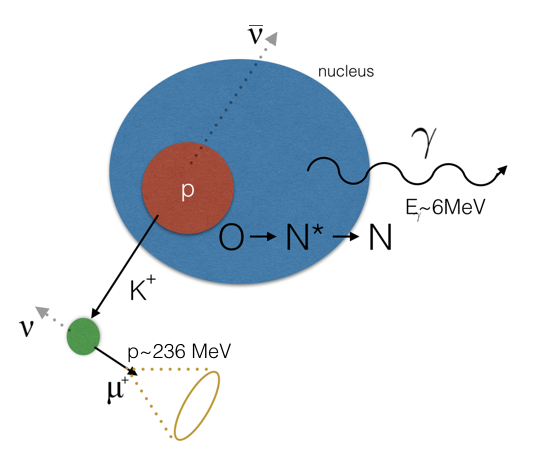
\includegraphics[width=0.37\linewidth]{figs/mugamma_mode.png}
  \caption{A proton inside an Oxygen nucleus decays to $\bar{\nu} + K^{+}$ and the remaining nucleus emits a 6 MeV photon. Later the Kaon decays into a $\nu$  and a mono-energetic  $\mu^{+}$ of about 236 MeV.}
  \label{fig:pdecay}
\end{figure}

Even though the situation is better now, it is still a challenge to identify if a signal comes from a proton that decayed or a neutrino that entered the detector and interacted with some nucleus. There are billions\footnote{Neutrinos come from many different sources, the main ones are the atmosphere and the Sun. Most of them cross our bodies, the Earth and all else and leave intact, since the chance of a neutrino interacting with something is incredibly small. Only from the Sun, 65 billion neutrinos cross a  person's thumb every second.} of neutrinos entering the detector every second. The chance of a neutrino interacting with a nucleus inside the tank is extremely small, but since the flux of incoming neutrinos is so high, we are bound to see some neutrino events\footnote{The detection of neutrinos in SK was awarded the Nobel prize in physics in 2015 for proving that neutrinos have mass \cite{Nobel}.} every hour or so.

Some of these events leave a trace in the detector that is very similar to our signal, so distinguishing between signal and background events is challenging. SK has searched for this decay mode before and the strategy used was to apply simple cuts in reconstructed variables such as momentum and number of particles present in the event \cite{Miura}. By looking at many distributions of these variables (features) and applying hard boundary cuts on them, a selection criteria was used to determine if an event is coming from signal or background.

The rejection of background events is already very powerful in the standard analysis, however it would be better if it could be further improved. Due to the fact that proton decay was never observed, it is crucial to reduce the number of False Positives as much as possible so that if an event is detected, we are confident that it comes from proton decay and not background. Even if no event is seen in the data, a lower limit for the proton lifetime can be calculated using a Poisson distribution. Increasing this limit is important to further restrict GUT models based on their predictions for the proton lifetime.

The goal of this study is to improve the selection criteria for this proton decay mode using Machine Learning techniques. This could enhance the signal-background separation leading to a better limit on the proton lifetime or ultimately the discovery of proton decay. This would be a huge discovery that will certainly change the current view of particle physics and deeper our knowledge of elementary particles and the fundamental interactions of nature. 



\section{Datasets and Inputs} \label{Data}

We will use 2 sets of data in this project, one for each class to be classified. Both sets are similarly generated using many steps of simulation. The first step is to generate the events using Monte Carlo event generators. The generator used in SK for neutrino interactions is called NEUT \ref{NEUT} and the proton decay generator is a custom code of the collaboration that simply generates a vector of kinematic variables for each particle present in the decay.

Once the events are generated, it is necessary to do the detector simulation part. This is where we simulate how the particles created in the first step will interact as they travel through the water inside the SK tank. This code is also a custom simulator called skdetsim, which is based on a general package called Geant3 \ref{Geant}. Finally, once all the physics simulation is done, the events need to be reconstructed, this is called event reconstruction. SK has 2 main algorithms to perform event reconstruction, APFit and fiTQun. In this study we will use fiTQun, it uses a maximum likelihood  method based on different hypotheses for an event to reconstruct the kinematics of all particles present in the event.

After all these steps, we have a labelled data set containing many features for every particle present in the event and the label tells us if it was a generated by a simulation of proton decay (class 1) or neutrino interaction (class 0) events. A pre-selection criteria will be applied in the data before we start the analysis. These cuts are necessary to guarantee that fiTQun will perform well, namely, we will only use events that are fully contained inside the fiducial volume (FCFV) of the tank\footnote{This means that the event started and ended inside the detector and 2 m away from the tank walls, without any activity happening outside.}. Also, we need 1-ring events, which means that at most only one particle is detected at a time. This is because our signal is the mono-energetic muon and the low energy photon. The photon energy is so small that it will not produce enough light to be seen as a Cherenkov ring in the detector, while the muon will be clearly seen. Therefore, we can reduce a lot of background by only looking at events that contain only one particle.

Once this pre-selection is applied we can finally start using ML to optimize our event classification. The different features we plan to use in the analysis are:
\begin{itemize}  
\item  $\ln{\left(\frac{L_{\mu}}{L_{e}}\right)}$: This is the log of the ratio of likelihoods for the electron and muon hypotheses. FiTQun will try to fit the event using a electron as the hypothesis and using a muon, for each fit we have the likelihood of how good the fit is, similar to a goodness of fit. We can then compare the likelihood of different hypotheses to see which one is more likely.
\item  $\ln{\left(\frac{L_{\mu}}{L_{\pi}}\right)}$: Similarly, we can compare the likelihood of the ring being created by a muon and a charged pion.
\item  $\ln{\left(\frac{L_{\mu}}{L_{\mu\gamma}}\right)}$: And finally, we can compare the likelihood of the event having a single muon present or a low energy photon being also present.
\item $P_{\mu}$: This is the reconstructed momentum\footnote{In high energy physics the unit of energy and momentum used is the electronVolt (eV), such that 1 MeV is 1 million eV.} of the muon.
\item $P_{\gamma}$: The reconstructed momentum of the photon.
\item $\Delta T$: The time difference between the muon ring appearing and the photon, in the hypothesis where both are present in the event. Ideally, for signal events this would have a non-zero time difference between them, since the Kaon travels some time before decaying. For neutrino events, the muon is produced instantaneously, so the time difference should be close to zero.
\item  $\Delta X$: The distance between the muon and the Michel electron\footnote{Michel electron is the electron that comes after the muon decays \ref{Michel}.} vertices. 
\end{itemize}

The proton decay sample generated contains 100,000 events, out of which approximately 30,000 are events where the Kaon decayed to a muon and the low energy photon was present. After applying the pre-selection cuts of only FCFV 1-ring events, the number goes down do about 22,000 events.
The atmospheric neutrino event sample was generated using 500 years of Monte Carlo simulation. This means that we simulate a number of events equivalent to SK running for 500 years without stopping. Neutrino interactions are so rare, that a huge amount of events are necessary to be able to properly estimate the number of events in a low-background search like ours. The total number of neutrino events is on the order of 2.5 million events. After applying pre-selection cuts, the number of background events is still very big.

A filter was selected to treat the data a bit more. Some cuts were already applied to all events using some of the described features above. This way, the number of background events is drastically reduced while the number of signal events is still high. These cuts are loose, in the sense that still a very high number of background events are passing them. The goal is just to reduce the amount of events so that the signal and background samples have a similar number of events. The choice of these cuts are also chosen based on physics prior, we know that the final analysis must have more strict cuts than these. So it will not bias our results if we only look at these neutrino background events. It is guaranteed that the events that are left out here will never be mistaken as signal events. Details of pre-selection will not be provided here since they are not the main purpose of this study. The definition of pre-selection cuts is:

\begin{itemize} 
\item $\ln{\left(\frac{L_{\mu}}{L_{e}}\right) > 0}$: Events should look more like muons than electrons.
\item $210 \textrm{ MeV} < P_{\mu} < 270 \textrm{ MeV}$: The muon momentum is known to be about 236 MeV, due to detector limitations, we can not measure momentum with infinite resolution. Therefore a window around the expected momentum is allowed.
\item $P_{\gamma} < 2 \textrm{ MeV}$: The momentum of the photon should be at least 2 MeV. This will get rid of events where no photon is found.
\item $\Delta T > 0 \textrm{ ns}$: The time difference between the muon and the photon should be at least 0 nanoseconds. We know that the muon will come after the photon in our signal, so we get rid of a lot of background that has negative $\Delta T$ values.
\end{itemize}

After applying this filter we are finally ready to begin being analyzed. We still have to prepare the data further before feeding it to some ML algorithm, like standardizing each feature, etc. But this will be done in the final project submission. Our final set of data contains 18652 signal events and 24435 neutrino events.


\section{Solution Statement}

As describe in section \ref{Data}, we can reduce the amount of background events by a factor of 100 already, keeping only the interesting neutrino events that can be mistaken as a proton decay signal increasing the false positive rate. But the number of background events remaining is still high and need to be reduced event further\footnote{Sections \ref{Benchmark} and \ref{Metric} describe why it is so important to have such a small number of false positives in this type of search.}.

Our goal here is to use machine learning algorithms to learn an optimized way of classifying events as signal or background. The way the standard analysis is done is by using a decision tree, since it simply applies boundary cuts on different features of the data. A natural choice of algorithm for the new analysis could be Boosted Decision Trees to continue in the same direction. Because of systematic uncertainties that have to be taken into account, dealing with boundary cuts can be a lot easier that dealing with complicated decisions, like the output of neural nets.

But since this approach is completely new, there is no reason to be attached to the standard way and new algorithms can be tested. The plan is to test different algorithms like for example Random Forest and Support Vector Machines. Both these algorithms can find a new boundary that separates both classes in feature space.
Applying a dimensionality reduction algorithm is something typical in ML applications, but it will not be used here. There are two main reasons for that, one is that our feature space is not that big compared to image recognition for instance, where the number of features is thousands of times bigger than ours. Also, we want to keep track of the features that are being used in the feature space itself, since they have a one-to-one mapping with physical quantities. If an algorithm like Principal Component Analysis is applied, the new space is a linear combination of the original features which complicates the interpretation of final results and dealing with systematic errors. The treatment of systematic uncertainties is beyond the purpose of this study, but it is necessary to keep it in mind when choosing an algorithm for the analysis.

Here we simply want find an algorithm with simple interpretation that performs well given some metric that will be discussed in Section \ref{Metric}. The goal is to perform better than the standard analysis and there are two ways this can be achieved. Either we improve the efficiency of keeping signal events while having the same amount of background events. Or we keep a similar efficiency while reducing the number of background by a factor of 2 or so. Of course, achieving both higher efficiency and reduced number of background is the best possible scenario. But if only one of them is achieved the effort can be considered a success. The definition of efficiency that will be used in this work is given by eq. \ref{eq:eff} in Section \ref{Benchmark}.


\section{Evaluation Metrics} \label{Metric}

In this section, propose at least one evaluation metric that can be used to quantify the performance of both the benchmark model and the solution model. The evaluation metric(s) you propose should be appropriate given the context of the data, the problem statement, and the intended solution. Describe how the evaluation metric(s) are derived and provide an example of their mathematical representations (if applicable). Complex evaluation metrics should be clearly defined and quantifiable (can be expressed in mathematical or logical terms).





\section{Benchmark Model} \label{Benchmark}

As discussed in Section \ref{Problem}, SK has already performed a search for the mode we are studying here. This particular mode is sometimes called prompt-gamma method, since it relies on the coincidence measurement of the muon and the photon that is promptly emitted by the nucleus. The details of the analysis, as well as the final results can be found in \cite{Miura}, but figure \ref{fig:benchmark} shows a table that summarizes the main results of that search.

\begin{figure}[h]
  \centering
  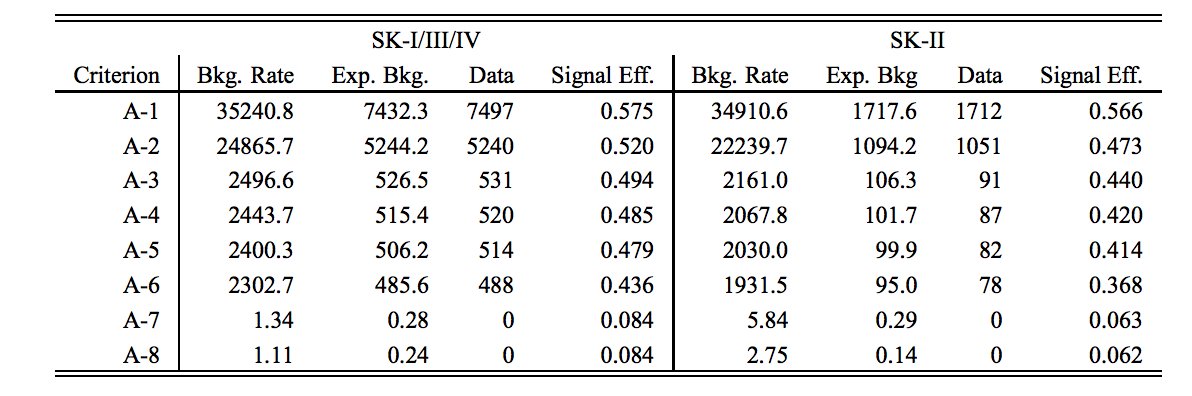
\includegraphics[width=0.8\linewidth]{figs/benchmark.png}
  \caption{Summary of the results obtained in the standard analysis done in SK. Definition of all quantities is given in the text.}
  \label{fig:benchmark}
\end{figure}

The criteria A1-8 are the different cuts applied in that analysis, the background rate is explained in more detail in Section \ref{Background}, eq. \ref{eq:mtonyear}, but basically it refers to the expected number of false positives if the detector had 1 million tones of volume and took data for 1 year. The expected background is the number of false positives in the analyzed data after each cut $\textrm{A}-i$ is applied, and the Data column corresponds to the actual number observed. 
Finally, the Signal Efficiency is defined in eq. \ref{eq:eff} in Section \ref{Efficiency} and corresponds to recall, i.e., the probability that an event is classified as signal given that it is signal.

The table contains values for all SK eras, from I to IV. SK-II is different due to an accident that reduced the number of PMTs, so the photo-coverage is different. We are using simulated data for SK-IV only, while the table contains the averaged results of SK I, III and IV. SK-IV performance if better than I and III due to better electronics and other factors,  but since the performance is not super different. We can use the numbers in the first column as our benchmark model.

The efficiency in the last column is reported to be 

\begin{equation} \label{eq:effB}
\epsilon_{B} = 0.084 = 8.4\%,
\end{equation}

where $B$ stands for Benchmark. This is one of the main numbers we wanna compare to, so using the definition of efficiency given in \ref{eq:eff} and the necessary scale factor discussed in Section \ref{Efficiency}, we can make a comparison between all classifiers used in this study and the benchmark model.

Also, since the amount of data analyzed will be different, we have to compare the number of false positives in our analysis with the $\textrm{Mton}\cdot\textrm{year}$ rate provided in the table. Section \ref{Background} explain the necessary transformations we need to do with FP to compare with the benchmark rate. Eq. \ref{eq:mtonyear} gives the rescale for our analysis and the benchmark result we can define as:

\begin{equation} \label{eq:MtonB}
R_{B} = 1.1\textrm{ event per Mega-tone per year}.
\end{equation}

Section \ref{Metric} discusses different metrics that will be used in this study. They will be useful when comparing different classifiers among themselves, but to compare our final results with the benchmark model provided by the standard analysis of SK, I will use the efficiency and rate defined here in eqs. \ref{eq:effB} and \ref{eq:MtonB}.



\section{Project Design}

In this final section, summarize a theoretical workflow for approaching a solution given the problem. Provide thorough discussion for what strategies you may consider employing, what analysis of the data might be required before being used, or which algorithms will be considered for your implementation. The workflow and discussion that you provide should align with the qualities of the previous sections. Additionally, you are encouraged to include small visualizations, pseudocode, or diagrams to aid in describing the project design, but it is not required. The discussion should clearly outline your intended workflow of the capstone project.


\section{Before submitting your proposal, ask yourself. . .}

\begin{itemize}  
\item Does the proposal you have written follow a well-organized structure similar to that of the project template?
 
\item Is each section (particularly Solution Statement and Project Design) written in a clear, concise and specific fashion? Are there any ambiguous terms or phrases that need clarification?
 
\item Would the intended audience of your project be able to understand your proposal?

\item Have you properly proofread your proposal to assure there are minimal grammatical and spelling mistakes?

\item Are all the resources used for this project correctly cited and referenced?

\ldots 
\end{itemize}

\begin{thebibliography}{9}

\bibitem{GUTs}
  W. de Boer,
  \textbf{Grand Unified Theories
	and Supersymmetry in
	Particle Physics and Cosmology}.
  \href{https://arxiv.org/pdf/hep-ph/9402266.pdf}{arXiv:9402266}

\bibitem{SK}
  Super-Kamiokande collaboration,
  \textbf{The Super-Kamiokande detector},
  Nuclear Instruments and Methods in Physics Research A 501 (2003) 418-462. 
  \href{http://www-sk.icrr.u-tokyo.ac.jp/~masato_s/class/sk-detector.pdf}{SK detector}
  
  \bibitem{Cherenkov}
  For more see: 
  \href{https://en.wikipedia.org/wiki/Cherenkov_radiation}{Wiki Cherenkov Radiation}

  \bibitem{PMT}
  For more see: 
  \href{https://en.wikipedia.org/wiki/Photomultiplier}{Wiki Photomultipliers}
  
  \bibitem{Nobel}
  For more see: 
  \href{http://www.nobelprize.org/nobel_prizes/physics/laureates/2015/}{2015 Nobel}
  
  \bibitem{Miura}
  Super-Kamiokande collaboration,
  \textbf{Search for Proton Decay via $p\rightarrow \nu K^{+}$ using 260 kiloton$\cdot$year data of Super-Kamiokande}.
  \href{https://arxiv.org/pdf/1408.1195v1.pdf}{arXiv:1408.1195}
  
  \bibitem{NEUT}
  Y. Hayato,
   \textbf{A neutrino interaction simulation program library NEUT}.
  \href{http://inspirehep.net/record/844435/files/v40p2477.pdf?version=1}{NEUT}
  
  \bibitem{Geant}
  Geant can be downloaded from: 
  \href{https://root.cern.ch/installing-geant3}{Geant}
  
  \bibitem{Michel}
  For more:
  \href{https://en.wikipedia.org/wiki/Michel_parameters}{Wiki Michel Electron}
  
  \bibitem{Nobel2}
  For more:
  \href{http://www.nobelprize.org/nobel_prizes/physics/laureates/2015/}{2015 Nobel}


\end{thebibliography}



\end{document}

